\documentclass{whiteboard}
\begin{document}
\begin{frame}[plain,t]
\bbcover{SPOJ IITKWPCG}{Help the old King}{Prof. Edson Alves}{Faculdade UnB Gama}

\end{frame}
\begin{frame}[plain,t]
\vspace*{\fill}

\bbenglish{Once upon a time there lived a king in a far far country. In the country, there are $n$ cities and $m$ roads. He was severly attacked by his enemy. The enemy damaged all the cities of King's country. As the roads between the cities had been damaged, the King wanted to repair those. So he decided to launch a tender for this.}

\vspace{0.1in}

\bbenglish{As King's country is a well managed country. By well managed country, we mean that it is possible to go from each city to any other city. But now as the city has been destroyed by enemies, all the roads are broken, the king will like to rebuild the roads in such a way that it is still a well manged country.}

\vspace{0.1in}

\bbenglish{Cost of repairing the road in the country is really wierd, it is not addition of costs but it is instead multiplication of those. What it means that if the king decides that he should repair $5$ roads, then total cost of repairing those roads will be multiplication of all the $5$ costs.}

\vspace*{\fill}
\end{frame}
\begin{frame}[plain,t]
\vspace*{\fill}

\bbtext{Era uma vez um rei que vivia em um reino muito, muito distante. Neste reino há $n$ povoados e $m$ estradas. O rei foi atacado severamente por seu inimigo. O inimigo danificou todos os povoados do reino. Uma vez que as estradas entre os povoados foram danificadas, o rei quer reparar estas estradas. Deste modo, ele decidiu lançar uma proposta para isto.}

\vspace{0.1in}

\bbtext{O reino é bem planejado, e por bem planejado entenda que é possível ir de qualquer povoado a qualquer outro povoado. Mas como os povooados foram destruídas por inimigos, todas as estradas estão em ruínas, o rei irá reconstruir as estradas de modo que o reino se torne novamente um reino bem planejado.}

\vspace{0.1in}

\bbtext{O custo de reparo de uma estrada neste reino é realmente estranho, de modo que ele não adiciona ao custo total, e sim multiplica. Isto significa que se o rei decidir reparar $5$ estradas, então o custo total do reparo destas estradas será a multiplicação dos $5$ custos individuais de cada estrada.}

\vspace*{\fill}
\end{frame}
\begin{frame}[plain,t]
\vspace*{\fill}

\bbenglish{As the King's treasure has been damaged by the attack of foreign city, he would like to spend minimum amount of money and that the will want that his country still remains well managed country. Surprisingly the company that was given tender had a rule that all the costs will be in powers of two, as they were really love with binary numbers.}

\vspace{0.1in}

\bbenglish{As value of the total cost can be really large. We do not want to know the actual cost, instead output number of divisors of the number.}

\vspace*{\fill}
\end{frame}
\begin{frame}[plain,t]
\vspace*{\fill}

\bbtext{Uma vez que o tesouro real foi prejudicado pelo ataque estrangeiro, o rei gostaria de gastar o mínimo possível de dinheiro e ele deseja que o país continue sendo bem planejado. Supreendentemente, a compania que assumiu a proposta tem uma regra que todos os custos serão potências de dois, uma vez que eles realmente gostam de números binários.}

\vspace{0.1in}

\bbtext{Uma vez que o custo total pode ser muito grande, nos não desejamos este valor. Ao invés disso, imprima o número de divisores deste valor.}

\vspace*{\fill}
\end{frame}
\begin{frame}[plain,t]
\vspace*{\fill}

\bbbold{Input}

\vspace{0.1in}

\bbenglish{$T$: number of test cases $(T \leq 5)$}

\vspace{0.1in}

\bbenglish{$n$ and $m$ $(n \leq 10^5$ \&\& $m \leq 2 \times 10^5)$}

\vspace{0.1in}

\bbenglish{Next $m$ lines will have $a, b, c$, which denotes that cities $a$ and $b$ are connected with road of cost $c$.}

\vspace{0.1in}

\bbenglish{$(c \geq 2$ \&\& $c \leq 10^{18}$ \&\& $c$ will always be power of $2)$ $(1 \leq a \leq n)$ and $(1 \leq b \leq n)$}

\vspace{0.2in}

\bbbold{Output}

\vspace{0.1in}

\bbenglish{For each test case, output a single line containing a number as stated in the problem.}

\vspace*{\fill}
\end{frame}
\begin{frame}[plain,t]
\vspace*{\fill}

\bbbold{Entrada}

\vspace{0.1in}

\bbtext{$T$: número de casos de teste $(T \leq 5)$}

\vspace{0.1in}

\bbtext{$n$ e $m$ $(n \leq 10^5$ \&\& $m \leq 2 \times 10^5)$}

\vspace{0.1in}

\bbtext{As $m$ linhas seguintes terão inteiros $a, b, c$, os quais indicam que os povoados $a$ e $b$ estão conectadas por uma estrada de custo $c$.}

\vspace{0.1in}

\bbtext{$(c \geq 2$ \&\& $c \leq 10^{18}$ \&\& $c$ será sempre uma potência de $2)$ $(1 \leq a \leq n)$ e $(1 \leq b \leq n)$}

\vspace{0.2in}

\bbbold{Saída}

\vspace{0.1in}

\bbtext{Para cada caso de teste, imprima uma única linha contendo o número solicitado pelo problema.}

\vspace*{\fill}
\end{frame}
\begin{frame}[plain,t]
\begin{tikzpicture}
\node[draw,opacity=0] at (0, 0) {x};
\node[draw,opacity=0] at (14, 8) {x};

	\node[anchor=west] (header) at (0, 7.0) { \bbbold{Exemplo de entrada e saída} };

\end{tikzpicture}
\end{frame}
\begin{frame}[plain,t]
\begin{tikzpicture}
\node[draw,opacity=0] at (0, 0) {x};
\node[draw,opacity=0] at (14, 8) {x};

	\node[anchor=west] (header) at (0, 7.0) { \bbbold{Exemplo de entrada e saída} };


	\node[anchor=west] (line1) at (1.0, 6.0) { \bbtext{\texttt{2 1} } };

\end{tikzpicture}
\end{frame}
\begin{frame}[plain,t]
\begin{tikzpicture}
\node[draw,opacity=0] at (0, 0) {x};
\node[draw,opacity=0] at (14, 8) {x};

	\node[anchor=west] (header) at (0, 7.0) { \bbbold{Exemplo de entrada e saída} };


	\node[anchor=west] (line1) at (1.0, 6.0) { \bbtext{\texttt{2 1} } };


	\draw[->,color=BBViolet] (1.25, 5.0) to  (1.25, 5.75);

	\node[] (r) at (1.25, 4.75) { \footnotesize \bbcomment{\# de povoados} };

\end{tikzpicture}
\end{frame}
\begin{frame}[plain,t]
\begin{tikzpicture}
\node[draw,opacity=0] at (0, 0) {x};
\node[draw,opacity=0] at (14, 8) {x};

	\node[anchor=west] (header) at (0, 7.0) { \bbbold{Exemplo de entrada e saída} };


	\node[anchor=west] (line1) at (1.0, 6.0) { \bbtext{\texttt{2 1} } };


	\draw[->,color=BBViolet] (1.65, 5.0) to  (1.65, 5.75);

	\node[] (r) at (1.65, 4.75) { \footnotesize \bbcomment{\# de estradas} };



\end{tikzpicture}
\end{frame}
\begin{frame}[plain,t]
\begin{tikzpicture}
\node[draw,opacity=0] at (0, 0) {x};
\node[draw,opacity=0] at (14, 8) {x};

	\node[anchor=west] (header) at (0, 7.0) { \bbbold{Exemplo de entrada e saída} };


	\node[anchor=west] (line1) at (1.0, 6.0) { \bbtext{\texttt{2 1} } };







	\node[draw,very thick,circle] (node1) at (7.0, 4.0) { \bbtext{1} };

	\node[draw,very thick,circle] (node2) at (12.0, 4.0) { \bbtext{2} };
\end{tikzpicture}
\end{frame}
\begin{frame}[plain,t]
\begin{tikzpicture}
\node[draw,opacity=0] at (0, 0) {x};
\node[draw,opacity=0] at (14, 8) {x};

	\node[anchor=west] (header) at (0, 7.0) { \bbbold{Exemplo de entrada e saída} };


	\node[anchor=west] (line1) at (1.0, 6.0) { \bbtext{\texttt{2 1} } };


	\draw[->,color=BBViolet] (1.25, 4.25) to  (1.25, 5.25);

	\node[] (r) at (1.25, 4.0) { \footnotesize \bbcomment{povoado $a$} };




	\node[draw,very thick,circle] (node1) at (7.0, 4.0) { \bbtext{1} };

	\node[draw,very thick,circle] (node2) at (12.0, 4.0) { \bbtext{2} };

	\node[anchor=west] (line2) at (1.0, 5.5) { \bbtext{\texttt{1 2 16} } };



\end{tikzpicture}
\end{frame}
\begin{frame}[plain,t]
\begin{tikzpicture}
\node[draw,opacity=0] at (0, 0) {x};
\node[draw,opacity=0] at (14, 8) {x};

	\node[anchor=west] (header) at (0, 7.0) { \bbbold{Exemplo de entrada e saída} };


	\node[anchor=west] (line1) at (1.0, 6.0) { \bbtext{\texttt{2 1} } };


	\draw[->,color=BBViolet] (1.65, 4.25) to  (1.65, 5.25);

	\node[] (r) at (1.65, 4.0) { \footnotesize \bbcomment{povoado $b$} };




	\node[draw,very thick,circle] (node1) at (7.0, 4.0) { \bbtext{1} };

	\node[draw,very thick,circle] (node2) at (12.0, 4.0) { \bbtext{2} };

	\node[anchor=west] (line2) at (1.0, 5.5) { \bbtext{\texttt{1 2 16} } };





\end{tikzpicture}
\end{frame}
\begin{frame}[plain,t]
\begin{tikzpicture}
\node[draw,opacity=0] at (0, 0) {x};
\node[draw,opacity=0] at (14, 8) {x};

	\node[anchor=west] (header) at (0, 7.0) { \bbbold{Exemplo de entrada e saída} };


	\node[anchor=west] (line1) at (1.0, 6.0) { \bbtext{\texttt{2 1} } };


	\draw[->,color=BBViolet] (2.05, 4.25) to  (2.05, 5.25);

	\node[] (r) at (2.05, 4.0) { \footnotesize \bbcomment{custo do reparo $c$} };




	\node[draw,very thick,circle] (node1) at (7.0, 4.0) { \bbtext{1} };

	\node[draw,very thick,circle] (node2) at (12.0, 4.0) { \bbtext{2} };

	\node[anchor=west] (line2) at (1.0, 5.5) { \bbtext{\texttt{1 2 16} } };







\end{tikzpicture}
\end{frame}
\begin{frame}[plain,t]
\begin{tikzpicture}
\node[draw,opacity=0] at (0, 0) {x};
\node[draw,opacity=0] at (14, 8) {x};

	\node[anchor=west] (header) at (0, 7.0) { \bbbold{Exemplo de entrada e saída} };


	\node[anchor=west] (line1) at (1.0, 6.0) { \bbtext{\texttt{2 1} } };







	\node[draw,very thick,circle] (node1) at (7.0, 4.0) { \bbtext{1} };

	\node[draw,very thick,circle] (node2) at (12.0, 4.0) { \bbtext{2} };

	\node[anchor=west] (line2) at (1.0, 5.5) { \bbtext{\texttt{1 2 16} } };








	\draw[very thick](node1) to node[above] { \bbinfo{16} } (node2);

\end{tikzpicture}
\end{frame}
\begin{frame}[plain,t]
\begin{tikzpicture}
\node[draw,opacity=0] at (0, 0) {x};
\node[draw,opacity=0] at (14, 8) {x};

	\node[anchor=west] (header) at (0, 7.0) { \bbbold{Exemplo de entrada e saída} };


	\node[anchor=west] (line1) at (1.0, 6.0) { \bbtext{\texttt{2 1} } };







	\node[draw,very thick,circle] (node1) at (7.0, 4.0) { \bbtext{1} };

	\node[draw,very thick,circle] (node2) at (12.0, 4.0) { \bbtext{2} };

	\node[anchor=west] (line2) at (1.0, 5.5) { \bbtext{\texttt{1 2 16} } };








	\draw[very thick,color=BBCyan,dashed](node1) to node[above] { \bbinfo{16} } (node2);



\end{tikzpicture}
\end{frame}
\begin{frame}[plain,t]
\begin{tikzpicture}
\node[draw,opacity=0] at (0, 0) {x};
\node[draw,opacity=0] at (14, 8) {x};

	\node[anchor=west] (header) at (0, 7.0) { \bbbold{Exemplo de entrada e saída} };


	\node[anchor=west] (line1) at (1.0, 6.0) { \bbtext{\texttt{2 1} } };







	\node[draw,very thick,circle] (node1) at (7.0, 4.0) { \bbtext{1} };

	\node[draw,very thick,circle] (node2) at (12.0, 4.0) { \bbtext{2} };

	\node[anchor=west] (line2) at (1.0, 5.5) { \bbtext{\texttt{1 2 16} } };








	\draw[very thick,color=BBCyan,dashed](node1) to node[above] { \bbinfo{16} } (node2);




	\node[] (r) at (1.65, 4.0) { \bbinfo{5} };

	\draw[color=BBBlack,-latex,very thick] (1.65, 5.25) to  (1.65, 4.25);

\end{tikzpicture}
\end{frame}
\begin{frame}[plain,t]
\begin{tikzpicture}
\node[draw,opacity=0] at (0, 0) {x};
\node[draw,opacity=0] at (14, 8) {x};

	\node[anchor=west] (header) at (0, 7.0) { \bbbold{Exemplo de entrada e saída} };

\end{tikzpicture}
\end{frame}
\begin{frame}[plain,t]
\begin{tikzpicture}
\node[draw,opacity=0] at (0, 0) {x};
\node[draw,opacity=0] at (14, 8) {x};

	\node[anchor=west] (header) at (0, 7.0) { \bbbold{Exemplo de entrada e saída} };


	\node[anchor=west] (line1) at (1.0, 6.0) { \bbtext{\texttt{5 5} } };

\end{tikzpicture}
\end{frame}
\begin{frame}[plain,t]
\begin{tikzpicture}
\node[draw,opacity=0] at (0, 0) {x};
\node[draw,opacity=0] at (14, 8) {x};

	\node[anchor=west] (header) at (0, 7.0) { \bbbold{Exemplo de entrada e saída} };


	\node[anchor=west] (line1) at (1.0, 6.0) { \bbtext{\texttt{5 5} } };


	\node[draw,very thick,circle] (a) at (7.0, 4.0) { \bbtext{1} };

	\node[draw,very thick,circle] (b) at (10.0, 7.0) { \bbtext{2} };

	\node[draw,very thick,circle] (c) at (13.0, 4.0) { \bbtext{3} };

	\node[draw,very thick,circle] (d) at (12.0, 1.0) { \bbtext{4} };

	\node[draw,very thick,circle] (e) at (8.0, 1.0) { \bbtext{5} };


\end{tikzpicture}
\end{frame}
\begin{frame}[plain,t]
\begin{tikzpicture}
\node[draw,opacity=0] at (0, 0) {x};
\node[draw,opacity=0] at (14, 8) {x};

	\node[anchor=west] (header) at (0, 7.0) { \bbbold{Exemplo de entrada e saída} };


	\node[anchor=west] (line1) at (1.0, 6.0) { \bbtext{\texttt{5 5} } };


	\node[draw,very thick,circle] (a) at (7.0, 4.0) { \bbtext{1} };

	\node[draw,very thick,circle] (b) at (10.0, 7.0) { \bbtext{2} };

	\node[draw,very thick,circle] (c) at (13.0, 4.0) { \bbtext{3} };

	\node[draw,very thick,circle] (d) at (12.0, 1.0) { \bbtext{4} };

	\node[draw,very thick,circle] (e) at (8.0, 1.0) { \bbtext{5} };



	\node[anchor=west] (line2) at (1.0, 5.5) { \bbtext{\texttt{1 2 2} } };

\end{tikzpicture}
\end{frame}
\begin{frame}[plain,t]
\begin{tikzpicture}
\node[draw,opacity=0] at (0, 0) {x};
\node[draw,opacity=0] at (14, 8) {x};

	\node[anchor=west] (header) at (0, 7.0) { \bbbold{Exemplo de entrada e saída} };


	\node[anchor=west] (line1) at (1.0, 6.0) { \bbtext{\texttt{5 5} } };


	\node[draw,very thick,circle] (a) at (7.0, 4.0) { \bbtext{1} };

	\node[draw,very thick,circle] (b) at (10.0, 7.0) { \bbtext{2} };

	\node[draw,very thick,circle] (c) at (13.0, 4.0) { \bbtext{3} };

	\node[draw,very thick,circle] (d) at (12.0, 1.0) { \bbtext{4} };

	\node[draw,very thick,circle] (e) at (8.0, 1.0) { \bbtext{5} };



	\node[anchor=west] (line2) at (1.0, 5.5) { \bbtext{\texttt{1 2 2} } };


	\draw[very thick](a) to node[above left] { \bbinfo{2} } (b);

\end{tikzpicture}
\end{frame}
\begin{frame}[plain,t]
\begin{tikzpicture}
\node[draw,opacity=0] at (0, 0) {x};
\node[draw,opacity=0] at (14, 8) {x};

	\node[anchor=west] (header) at (0, 7.0) { \bbbold{Exemplo de entrada e saída} };


	\node[anchor=west] (line1) at (1.0, 6.0) { \bbtext{\texttt{5 5} } };


	\node[draw,very thick,circle] (a) at (7.0, 4.0) { \bbtext{1} };

	\node[draw,very thick,circle] (b) at (10.0, 7.0) { \bbtext{2} };

	\node[draw,very thick,circle] (c) at (13.0, 4.0) { \bbtext{3} };

	\node[draw,very thick,circle] (d) at (12.0, 1.0) { \bbtext{4} };

	\node[draw,very thick,circle] (e) at (8.0, 1.0) { \bbtext{5} };



	\node[anchor=west] (line2) at (1.0, 5.5) { \bbtext{\texttt{1 2 2} } };


	\draw[very thick](a) to node[above left] { \bbinfo{2} } (b);


	\node[anchor=west] (line3) at (1.0, 5.0) { \bbtext{\texttt{2 3 2 } } };

\end{tikzpicture}
\end{frame}
\begin{frame}[plain,t]
\begin{tikzpicture}
\node[draw,opacity=0] at (0, 0) {x};
\node[draw,opacity=0] at (14, 8) {x};

	\node[anchor=west] (header) at (0, 7.0) { \bbbold{Exemplo de entrada e saída} };


	\node[anchor=west] (line1) at (1.0, 6.0) { \bbtext{\texttt{5 5} } };


	\node[draw,very thick,circle] (a) at (7.0, 4.0) { \bbtext{1} };

	\node[draw,very thick,circle] (b) at (10.0, 7.0) { \bbtext{2} };

	\node[draw,very thick,circle] (c) at (13.0, 4.0) { \bbtext{3} };

	\node[draw,very thick,circle] (d) at (12.0, 1.0) { \bbtext{4} };

	\node[draw,very thick,circle] (e) at (8.0, 1.0) { \bbtext{5} };



	\node[anchor=west] (line2) at (1.0, 5.5) { \bbtext{\texttt{1 2 2} } };


	\draw[very thick](a) to node[above left] { \bbinfo{2} } (b);


	\node[anchor=west] (line3) at (1.0, 5.0) { \bbtext{\texttt{2 3 2 } } };


	\draw[very thick](c) to node[above right] { \bbinfo{2} } (b);

\end{tikzpicture}
\end{frame}
\begin{frame}[plain,t]
\begin{tikzpicture}
\node[draw,opacity=0] at (0, 0) {x};
\node[draw,opacity=0] at (14, 8) {x};

	\node[anchor=west] (header) at (0, 7.0) { \bbbold{Exemplo de entrada e saída} };


	\node[anchor=west] (line1) at (1.0, 6.0) { \bbtext{\texttt{5 5} } };


	\node[draw,very thick,circle] (a) at (7.0, 4.0) { \bbtext{1} };

	\node[draw,very thick,circle] (b) at (10.0, 7.0) { \bbtext{2} };

	\node[draw,very thick,circle] (c) at (13.0, 4.0) { \bbtext{3} };

	\node[draw,very thick,circle] (d) at (12.0, 1.0) { \bbtext{4} };

	\node[draw,very thick,circle] (e) at (8.0, 1.0) { \bbtext{5} };



	\node[anchor=west] (line2) at (1.0, 5.5) { \bbtext{\texttt{1 2 2} } };


	\draw[very thick](a) to node[above left] { \bbinfo{2} } (b);


	\node[anchor=west] (line3) at (1.0, 5.0) { \bbtext{\texttt{2 3 2 } } };


	\draw[very thick](c) to node[above right] { \bbinfo{2} } (b);


	\node[anchor=west] (line4) at (1.0, 4.5) { \bbtext{\texttt{1 3 4} } };

\end{tikzpicture}
\end{frame}
\begin{frame}[plain,t]
\begin{tikzpicture}
\node[draw,opacity=0] at (0, 0) {x};
\node[draw,opacity=0] at (14, 8) {x};

	\node[anchor=west] (header) at (0, 7.0) { \bbbold{Exemplo de entrada e saída} };


	\node[anchor=west] (line1) at (1.0, 6.0) { \bbtext{\texttt{5 5} } };


	\node[draw,very thick,circle] (a) at (7.0, 4.0) { \bbtext{1} };

	\node[draw,very thick,circle] (b) at (10.0, 7.0) { \bbtext{2} };

	\node[draw,very thick,circle] (c) at (13.0, 4.0) { \bbtext{3} };

	\node[draw,very thick,circle] (d) at (12.0, 1.0) { \bbtext{4} };

	\node[draw,very thick,circle] (e) at (8.0, 1.0) { \bbtext{5} };



	\node[anchor=west] (line2) at (1.0, 5.5) { \bbtext{\texttt{1 2 2} } };


	\draw[very thick](a) to node[above left] { \bbinfo{2} } (b);


	\node[anchor=west] (line3) at (1.0, 5.0) { \bbtext{\texttt{2 3 2 } } };


	\draw[very thick](c) to node[above right] { \bbinfo{2} } (b);


	\node[anchor=west] (line4) at (1.0, 4.5) { \bbtext{\texttt{1 3 4} } };


	\draw[very thick](c) to node[above] { \bbinfo{4} } (a);

\end{tikzpicture}
\end{frame}
\begin{frame}[plain,t]
\begin{tikzpicture}
\node[draw,opacity=0] at (0, 0) {x};
\node[draw,opacity=0] at (14, 8) {x};

	\node[anchor=west] (header) at (0, 7.0) { \bbbold{Exemplo de entrada e saída} };


	\node[anchor=west] (line1) at (1.0, 6.0) { \bbtext{\texttt{5 5} } };


	\node[draw,very thick,circle] (a) at (7.0, 4.0) { \bbtext{1} };

	\node[draw,very thick,circle] (b) at (10.0, 7.0) { \bbtext{2} };

	\node[draw,very thick,circle] (c) at (13.0, 4.0) { \bbtext{3} };

	\node[draw,very thick,circle] (d) at (12.0, 1.0) { \bbtext{4} };

	\node[draw,very thick,circle] (e) at (8.0, 1.0) { \bbtext{5} };



	\node[anchor=west] (line2) at (1.0, 5.5) { \bbtext{\texttt{1 2 2} } };


	\draw[very thick](a) to node[above left] { \bbinfo{2} } (b);


	\node[anchor=west] (line3) at (1.0, 5.0) { \bbtext{\texttt{2 3 2 } } };


	\draw[very thick](c) to node[above right] { \bbinfo{2} } (b);


	\node[anchor=west] (line4) at (1.0, 4.5) { \bbtext{\texttt{1 3 4} } };


	\draw[very thick](c) to node[above] { \bbinfo{4} } (a);


	\node[anchor=west] (line5) at (1.0, 4.0) { \bbtext{\texttt{3 4 16} } };

\end{tikzpicture}
\end{frame}
\begin{frame}[plain,t]
\begin{tikzpicture}
\node[draw,opacity=0] at (0, 0) {x};
\node[draw,opacity=0] at (14, 8) {x};

	\node[anchor=west] (header) at (0, 7.0) { \bbbold{Exemplo de entrada e saída} };


	\node[anchor=west] (line1) at (1.0, 6.0) { \bbtext{\texttt{5 5} } };


	\node[draw,very thick,circle] (a) at (7.0, 4.0) { \bbtext{1} };

	\node[draw,very thick,circle] (b) at (10.0, 7.0) { \bbtext{2} };

	\node[draw,very thick,circle] (c) at (13.0, 4.0) { \bbtext{3} };

	\node[draw,very thick,circle] (d) at (12.0, 1.0) { \bbtext{4} };

	\node[draw,very thick,circle] (e) at (8.0, 1.0) { \bbtext{5} };



	\node[anchor=west] (line2) at (1.0, 5.5) { \bbtext{\texttt{1 2 2} } };


	\draw[very thick](a) to node[above left] { \bbinfo{2} } (b);


	\node[anchor=west] (line3) at (1.0, 5.0) { \bbtext{\texttt{2 3 2 } } };


	\draw[very thick](c) to node[above right] { \bbinfo{2} } (b);


	\node[anchor=west] (line4) at (1.0, 4.5) { \bbtext{\texttt{1 3 4} } };


	\draw[very thick](c) to node[above] { \bbinfo{4} } (a);


	\node[anchor=west] (line5) at (1.0, 4.0) { \bbtext{\texttt{3 4 16} } };


	\draw[very thick](c) to node[below right] { \bbinfo{16} } (d);

\end{tikzpicture}
\end{frame}
\begin{frame}[plain,t]
\begin{tikzpicture}
\node[draw,opacity=0] at (0, 0) {x};
\node[draw,opacity=0] at (14, 8) {x};

	\node[anchor=west] (header) at (0, 7.0) { \bbbold{Exemplo de entrada e saída} };


	\node[anchor=west] (line1) at (1.0, 6.0) { \bbtext{\texttt{5 5} } };


	\node[draw,very thick,circle] (a) at (7.0, 4.0) { \bbtext{1} };

	\node[draw,very thick,circle] (b) at (10.0, 7.0) { \bbtext{2} };

	\node[draw,very thick,circle] (c) at (13.0, 4.0) { \bbtext{3} };

	\node[draw,very thick,circle] (d) at (12.0, 1.0) { \bbtext{4} };

	\node[draw,very thick,circle] (e) at (8.0, 1.0) { \bbtext{5} };



	\node[anchor=west] (line2) at (1.0, 5.5) { \bbtext{\texttt{1 2 2} } };


	\draw[very thick](a) to node[above left] { \bbinfo{2} } (b);


	\node[anchor=west] (line3) at (1.0, 5.0) { \bbtext{\texttt{2 3 2 } } };


	\draw[very thick](c) to node[above right] { \bbinfo{2} } (b);


	\node[anchor=west] (line4) at (1.0, 4.5) { \bbtext{\texttt{1 3 4} } };


	\draw[very thick](c) to node[above] { \bbinfo{4} } (a);


	\node[anchor=west] (line5) at (1.0, 4.0) { \bbtext{\texttt{3 4 16} } };


	\draw[very thick](c) to node[below right] { \bbinfo{16} } (d);


	\node[anchor=west] (line6) at (1.0, 3.5) { \bbtext{\texttt{3 5 8} } };

\end{tikzpicture}
\end{frame}
\begin{frame}[plain,t]
\begin{tikzpicture}
\node[draw,opacity=0] at (0, 0) {x};
\node[draw,opacity=0] at (14, 8) {x};

	\node[anchor=west] (header) at (0, 7.0) { \bbbold{Exemplo de entrada e saída} };


	\node[anchor=west] (line1) at (1.0, 6.0) { \bbtext{\texttt{5 5} } };


	\node[draw,very thick,circle] (a) at (7.0, 4.0) { \bbtext{1} };

	\node[draw,very thick,circle] (b) at (10.0, 7.0) { \bbtext{2} };

	\node[draw,very thick,circle] (c) at (13.0, 4.0) { \bbtext{3} };

	\node[draw,very thick,circle] (d) at (12.0, 1.0) { \bbtext{4} };

	\node[draw,very thick,circle] (e) at (8.0, 1.0) { \bbtext{5} };



	\node[anchor=west] (line2) at (1.0, 5.5) { \bbtext{\texttt{1 2 2} } };


	\draw[very thick](a) to node[above left] { \bbinfo{2} } (b);


	\node[anchor=west] (line3) at (1.0, 5.0) { \bbtext{\texttt{2 3 2 } } };


	\draw[very thick](c) to node[above right] { \bbinfo{2} } (b);


	\node[anchor=west] (line4) at (1.0, 4.5) { \bbtext{\texttt{1 3 4} } };


	\draw[very thick](c) to node[above] { \bbinfo{4} } (a);


	\node[anchor=west] (line5) at (1.0, 4.0) { \bbtext{\texttt{3 4 16} } };


	\draw[very thick](c) to node[below right] { \bbinfo{16} } (d);


	\node[anchor=west] (line6) at (1.0, 3.5) { \bbtext{\texttt{3 5 8} } };


	\draw[very thick](c) to node[above left] { \bbinfo{8} } (e);

\end{tikzpicture}
\end{frame}
\begin{frame}[plain,t]
\begin{tikzpicture}
\node[draw,opacity=0] at (0, 0) {x};
\node[draw,opacity=0] at (14, 8) {x};

	\node[anchor=west] (header) at (0, 7.0) { \bbbold{Exemplo de entrada e saída} };


	\node[anchor=west] (line1) at (1.0, 6.0) { \bbtext{\texttt{5 5} } };


	\node[draw,very thick,circle] (a) at (7.0, 4.0) { \bbtext{1} };

	\node[draw,very thick,circle] (b) at (10.0, 7.0) { \bbtext{2} };

	\node[draw,very thick,circle] (c) at (13.0, 4.0) { \bbtext{3} };

	\node[draw,very thick,circle] (d) at (12.0, 1.0) { \bbtext{4} };

	\node[draw,very thick,circle] (e) at (8.0, 1.0) { \bbtext{5} };



	\node[anchor=west] (line2) at (1.0, 5.5) { \bbtext{\texttt{1 2 2} } };


	\draw[very thick,color=BBCyan,dashed](a) to node[above left] { \bbinfo{2} } (b);


	\node[anchor=west] (line3) at (1.0, 5.0) { \bbtext{\texttt{2 3 2 } } };


	\draw[very thick](c) to node[above right] { \bbinfo{2} } (b);


	\node[anchor=west] (line4) at (1.0, 4.5) { \bbtext{\texttt{1 3 4} } };


	\draw[very thick](c) to node[above] { \bbinfo{4} } (a);


	\node[anchor=west] (line5) at (1.0, 4.0) { \bbtext{\texttt{3 4 16} } };


	\draw[very thick](c) to node[below right] { \bbinfo{16} } (d);


	\node[anchor=west] (line6) at (1.0, 3.5) { \bbtext{\texttt{3 5 8} } };


	\draw[very thick](c) to node[above left] { \bbinfo{8} } (e);


\end{tikzpicture}
\end{frame}
\begin{frame}[plain,t]
\begin{tikzpicture}
\node[draw,opacity=0] at (0, 0) {x};
\node[draw,opacity=0] at (14, 8) {x};

	\node[anchor=west] (header) at (0, 7.0) { \bbbold{Exemplo de entrada e saída} };


	\node[anchor=west] (line1) at (1.0, 6.0) { \bbtext{\texttt{5 5} } };


	\node[draw,very thick,circle] (a) at (7.0, 4.0) { \bbtext{1} };

	\node[draw,very thick,circle] (b) at (10.0, 7.0) { \bbtext{2} };

	\node[draw,very thick,circle] (c) at (13.0, 4.0) { \bbtext{3} };

	\node[draw,very thick,circle] (d) at (12.0, 1.0) { \bbtext{4} };

	\node[draw,very thick,circle] (e) at (8.0, 1.0) { \bbtext{5} };



	\node[anchor=west] (line2) at (1.0, 5.5) { \bbtext{\texttt{1 2 2} } };


	\draw[very thick,color=BBCyan,dashed](a) to node[above left] { \bbinfo{2} } (b);


	\node[anchor=west] (line3) at (1.0, 5.0) { \bbtext{\texttt{2 3 2 } } };


	\draw[very thick,color=BBCyan,dashed](c) to node[above right] { \bbinfo{2} } (b);


	\node[anchor=west] (line4) at (1.0, 4.5) { \bbtext{\texttt{1 3 4} } };


	\draw[very thick](c) to node[above] { \bbinfo{4} } (a);


	\node[anchor=west] (line5) at (1.0, 4.0) { \bbtext{\texttt{3 4 16} } };


	\draw[very thick](c) to node[below right] { \bbinfo{16} } (d);


	\node[anchor=west] (line6) at (1.0, 3.5) { \bbtext{\texttt{3 5 8} } };


	\draw[very thick](c) to node[above left] { \bbinfo{8} } (e);




\end{tikzpicture}
\end{frame}
\begin{frame}[plain,t]
\begin{tikzpicture}
\node[draw,opacity=0] at (0, 0) {x};
\node[draw,opacity=0] at (14, 8) {x};

	\node[anchor=west] (header) at (0, 7.0) { \bbbold{Exemplo de entrada e saída} };


	\node[anchor=west] (line1) at (1.0, 6.0) { \bbtext{\texttt{5 5} } };


	\node[draw,very thick,circle] (a) at (7.0, 4.0) { \bbtext{1} };

	\node[draw,very thick,circle] (b) at (10.0, 7.0) { \bbtext{2} };

	\node[draw,very thick,circle] (c) at (13.0, 4.0) { \bbtext{3} };

	\node[draw,very thick,circle] (d) at (12.0, 1.0) { \bbtext{4} };

	\node[draw,very thick,circle] (e) at (8.0, 1.0) { \bbtext{5} };



	\node[anchor=west] (line2) at (1.0, 5.5) { \bbtext{\texttt{1 2 2} } };


	\draw[very thick,color=BBCyan,dashed](a) to node[above left] { \bbinfo{2} } (b);


	\node[anchor=west] (line3) at (1.0, 5.0) { \bbtext{\texttt{2 3 2 } } };


	\draw[very thick,color=BBCyan,dashed](c) to node[above right] { \bbinfo{2} } (b);


	\node[anchor=west] (line4) at (1.0, 4.5) { \bbtext{\texttt{1 3 4} } };


	\draw[very thick](c) to node[above] { \bbinfo{4} } (a);


	\node[anchor=west] (line5) at (1.0, 4.0) { \bbtext{\texttt{3 4 16} } };


	\draw[very thick](c) to node[below right] { \bbinfo{16} } (d);


	\node[anchor=west] (line6) at (1.0, 3.5) { \bbtext{\texttt{3 5 8} } };


	\draw[very thick,color=BBCyan,dashed](c) to node[above left] { \bbinfo{8} } (e);





\end{tikzpicture}
\end{frame}
\begin{frame}[plain,t]
\begin{tikzpicture}
\node[draw,opacity=0] at (0, 0) {x};
\node[draw,opacity=0] at (14, 8) {x};

	\node[anchor=west] (header) at (0, 7.0) { \bbbold{Exemplo de entrada e saída} };


	\node[anchor=west] (line1) at (1.0, 6.0) { \bbtext{\texttt{5 5} } };


	\node[draw,very thick,circle] (a) at (7.0, 4.0) { \bbtext{1} };

	\node[draw,very thick,circle] (b) at (10.0, 7.0) { \bbtext{2} };

	\node[draw,very thick,circle] (c) at (13.0, 4.0) { \bbtext{3} };

	\node[draw,very thick,circle] (d) at (12.0, 1.0) { \bbtext{4} };

	\node[draw,very thick,circle] (e) at (8.0, 1.0) { \bbtext{5} };



	\node[anchor=west] (line2) at (1.0, 5.5) { \bbtext{\texttt{1 2 2} } };


	\draw[very thick,color=BBCyan,dashed](a) to node[above left] { \bbinfo{2} } (b);


	\node[anchor=west] (line3) at (1.0, 5.0) { \bbtext{\texttt{2 3 2 } } };


	\draw[very thick,color=BBCyan,dashed](c) to node[above right] { \bbinfo{2} } (b);


	\node[anchor=west] (line4) at (1.0, 4.5) { \bbtext{\texttt{1 3 4} } };


	\draw[very thick](c) to node[above] { \bbinfo{4} } (a);


	\node[anchor=west] (line5) at (1.0, 4.0) { \bbtext{\texttt{3 4 16} } };


	\draw[very thick,color=BBCyan,dashed](c) to node[below right] { \bbinfo{16} } (d);


	\node[anchor=west] (line6) at (1.0, 3.5) { \bbtext{\texttt{3 5 8} } };


	\draw[very thick,color=BBCyan,dashed](c) to node[above left] { \bbinfo{8} } (e);






\end{tikzpicture}
\end{frame}
\begin{frame}[plain,t]
\begin{tikzpicture}
\node[draw,opacity=0] at (0, 0) {x};
\node[draw,opacity=0] at (14, 8) {x};

	\node[anchor=west] (header) at (0, 7.0) { \bbbold{Exemplo de entrada e saída} };


	\node[anchor=west] (line1) at (1.0, 6.0) { \bbtext{\texttt{5 5} } };


	\node[draw,very thick,circle] (a) at (7.0, 4.0) { \bbtext{1} };

	\node[draw,very thick,circle] (b) at (10.0, 7.0) { \bbtext{2} };

	\node[draw,very thick,circle] (c) at (13.0, 4.0) { \bbtext{3} };

	\node[draw,very thick,circle] (d) at (12.0, 1.0) { \bbtext{4} };

	\node[draw,very thick,circle] (e) at (8.0, 1.0) { \bbtext{5} };



	\node[anchor=west] (line2) at (1.0, 5.5) { \bbtext{\texttt{1 2 2} } };


	\draw[very thick,color=BBCyan,dashed](a) to node[above left] { \bbinfo{2} } (b);


	\node[anchor=west] (line3) at (1.0, 5.0) { \bbtext{\texttt{2 3 2 } } };


	\draw[very thick,color=BBCyan,dashed](c) to node[above right] { \bbinfo{2} } (b);


	\node[anchor=west] (line4) at (1.0, 4.5) { \bbtext{\texttt{1 3 4} } };


	\draw[very thick](c) to node[above] { \bbinfo{4} } (a);


	\node[anchor=west] (line5) at (1.0, 4.0) { \bbtext{\texttt{3 4 16} } };


	\draw[very thick,color=BBCyan,dashed](c) to node[below right] { \bbinfo{16} } (d);


	\node[anchor=west] (line6) at (1.0, 3.5) { \bbtext{\texttt{3 5 8} } };


	\draw[very thick,color=BBCyan,dashed](c) to node[above left] { \bbinfo{8} } (e);







	\node[] (r) at (1.65, 2.0) { \bbinfo{10} };

	\draw[color=BBBlack,-latex,very thick] (1.65, 3.25) to  (1.65, 2.25);

\end{tikzpicture}
\end{frame}
\begin{frame}[plain,t]
\begin{tikzpicture}
\node[draw,opacity=0] at (0, 0) {x};
\node[draw,opacity=0] at (14, 8) {x};

	\node[anchor=west] (title) at (0.0, 7.0) { \Large \bbbold{Solução} };
\end{tikzpicture}
\end{frame}
\begin{frame}[plain,t]
\begin{tikzpicture}
\node[draw,opacity=0] at (0, 0) {x};
\node[draw,opacity=0] at (14, 8) {x};

	\node[anchor=west] (title) at (0.0, 7.0) { \Large \bbbold{Solução} };

	\node[anchor=west] (a) at (1.0, 6.0) { $\star$ \bbtext{A MST minimiza também o produto dos pesos da arestas} };

\end{tikzpicture}
\end{frame}
\begin{frame}[plain,t]
\begin{tikzpicture}
\node[draw,opacity=0] at (0, 0) {x};
\node[draw,opacity=0] at (14, 8) {x};

	\node[anchor=west] (title) at (0.0, 7.0) { \Large \bbbold{Solução} };

	\node[anchor=west] (a) at (1.0, 6.0) { $\star$ \bbtext{A MST minimiza também o produto dos pesos da arestas} };


	\node[anchor=west] (b) at (1.0, 5.0) { $\star$ \bbtext{Para verificar este fato, basta substituir os pesos de $G$ por seus respectivos} };

	\node[anchor=west] (b1) at (0.5, 4.5) { \bbtext{logaritmos e identificar a MST do grafo $G'$ resultante} };

\end{tikzpicture}
\end{frame}
\begin{frame}[plain,t]
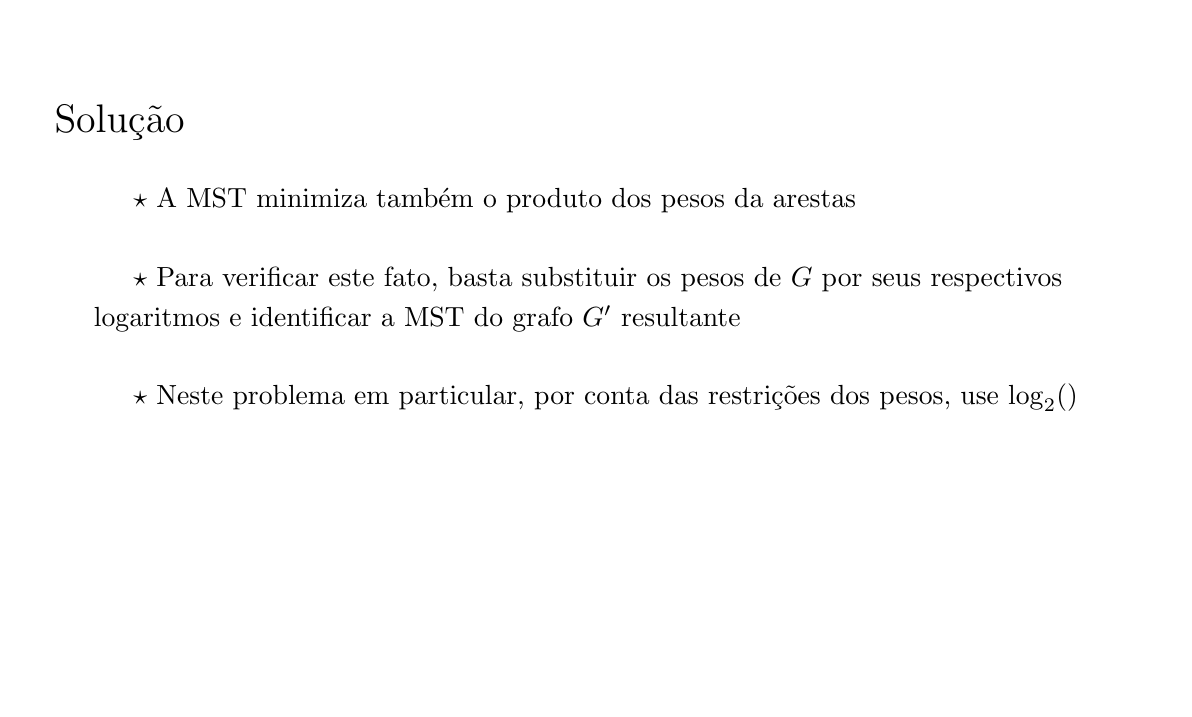
\begin{tikzpicture}
\node[draw,opacity=0] at (0, 0) {x};
\node[draw,opacity=0] at (14, 8) {x};

	\node[anchor=west] (title) at (0.0, 7.0) { \Large \bbbold{Solução} };

	\node[anchor=west] (a) at (1.0, 6.0) { $\star$ \bbtext{A MST minimiza também o produto dos pesos da arestas} };


	\node[anchor=west] (b) at (1.0, 5.0) { $\star$ \bbtext{Para verificar este fato, basta substituir os pesos de $G$ por seus respectivos} };

	\node[anchor=west] (b1) at (0.5, 4.5) { \bbtext{logaritmos e identificar a MST do grafo $G'$ resultante} };


	\node[anchor=west] (c) at (1.0, 3.5) { $\star$ \bbtext{Neste problema em particular, por conta das restrições dos pesos, use $\log_2()$} };

\end{tikzpicture}
\end{frame}
\begin{frame}[plain,t]
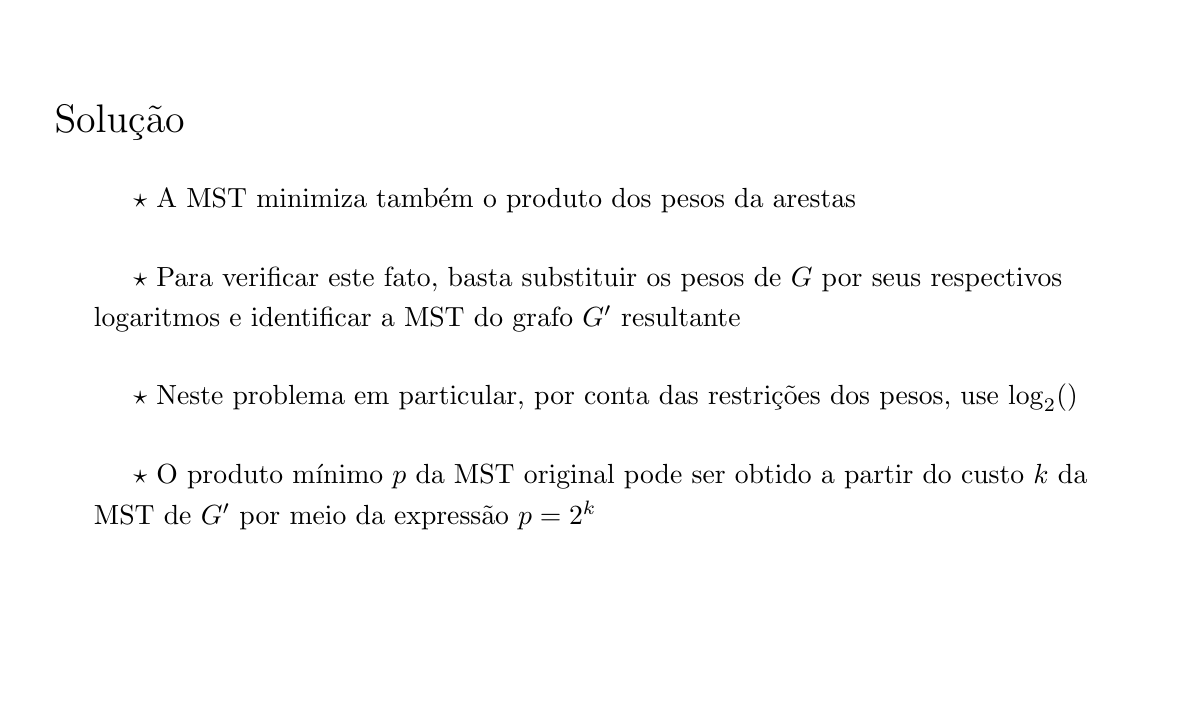
\begin{tikzpicture}
\node[draw,opacity=0] at (0, 0) {x};
\node[draw,opacity=0] at (14, 8) {x};

	\node[anchor=west] (title) at (0.0, 7.0) { \Large \bbbold{Solução} };

	\node[anchor=west] (a) at (1.0, 6.0) { $\star$ \bbtext{A MST minimiza também o produto dos pesos da arestas} };


	\node[anchor=west] (b) at (1.0, 5.0) { $\star$ \bbtext{Para verificar este fato, basta substituir os pesos de $G$ por seus respectivos} };

	\node[anchor=west] (b1) at (0.5, 4.5) { \bbtext{logaritmos e identificar a MST do grafo $G'$ resultante} };


	\node[anchor=west] (c) at (1.0, 3.5) { $\star$ \bbtext{Neste problema em particular, por conta das restrições dos pesos, use $\log_2()$} };


	\node[anchor=west] (d) at (1.0, 2.5) { $\star$ \bbtext{O produto mínimo $p$ da MST original pode ser obtido a partir do custo $k$ da} };

	\node[anchor=west] (d1) at (0.5, 2.0) { \bbtext{MST de $G'$ por meio da expressão $p = 2^k$} };

\end{tikzpicture}
\end{frame}
\begin{frame}[plain,t]
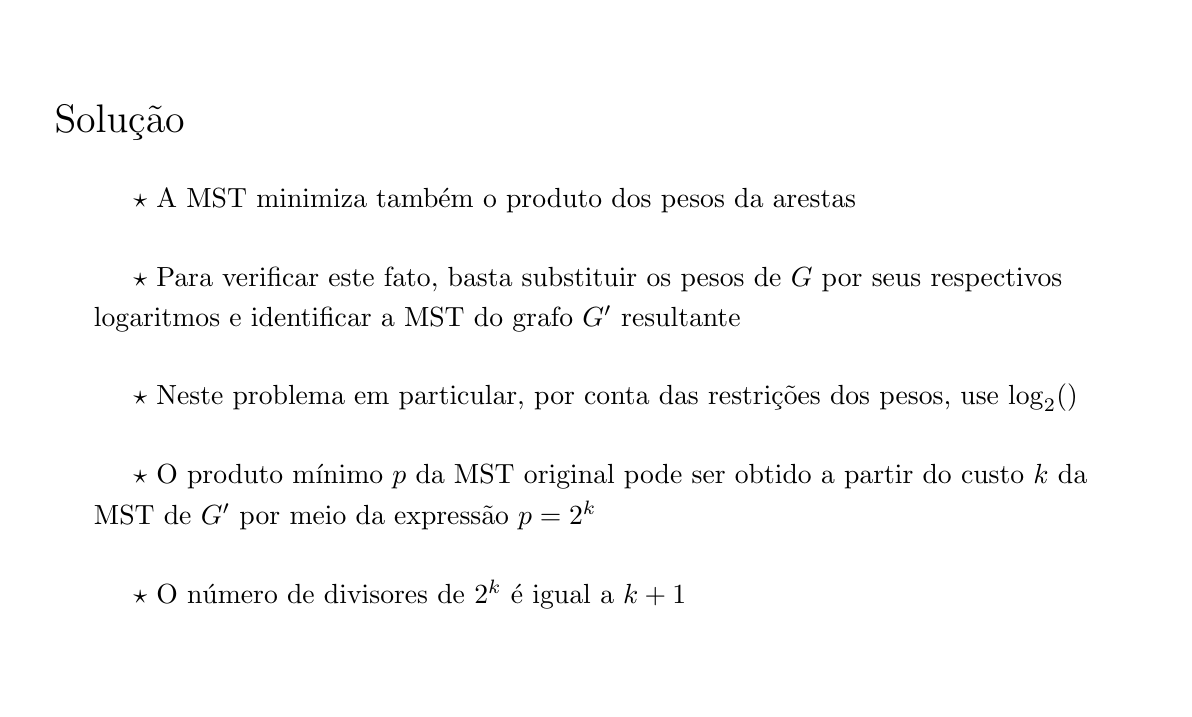
\begin{tikzpicture}
\node[draw,opacity=0] at (0, 0) {x};
\node[draw,opacity=0] at (14, 8) {x};

	\node[anchor=west] (title) at (0.0, 7.0) { \Large \bbbold{Solução} };

	\node[anchor=west] (a) at (1.0, 6.0) { $\star$ \bbtext{A MST minimiza também o produto dos pesos da arestas} };


	\node[anchor=west] (b) at (1.0, 5.0) { $\star$ \bbtext{Para verificar este fato, basta substituir os pesos de $G$ por seus respectivos} };

	\node[anchor=west] (b1) at (0.5, 4.5) { \bbtext{logaritmos e identificar a MST do grafo $G'$ resultante} };


	\node[anchor=west] (c) at (1.0, 3.5) { $\star$ \bbtext{Neste problema em particular, por conta das restrições dos pesos, use $\log_2()$} };


	\node[anchor=west] (d) at (1.0, 2.5) { $\star$ \bbtext{O produto mínimo $p$ da MST original pode ser obtido a partir do custo $k$ da} };

	\node[anchor=west] (d1) at (0.5, 2.0) { \bbtext{MST de $G'$ por meio da expressão $p = 2^k$} };


	\node[anchor=west] (e) at (1.0, 1.0) { $\star$ \bbtext{O número de divisores de $2^k$ é igual a $k + 1$} };


\end{tikzpicture}
\end{frame}
\begin{frame}[plain,t]

\inputsnippet{cpp}{41}{59}{codes/IITKWPCG.cpp}

\end{frame}
\end{document}
